\chapter{外文资料原文}
\label{cha:engorg}

\title{Deep Reinforcement Learning for Dynamic Multichannel Access in Wireless Networks }

\textbf{Abstract:} We consider a dynamic multichannel access problem, where multiple correlated channels follow an unknown joint Markov model and users select the channel to transmit data. The objective is to find a policy that maximizes the expected long-term number of successful transmissions. The problem is formulated as a partially observable Markov decision process with unknown system dynamics. To overcome the challenges of unknown dynamics and prohibitive computation, we apply the concept of reinforcement learning and implement a deep Q-network (DQN). We first study the optimal policy for fixedpattern channel switching with known system dynamics and show through simulations that DQN can achieve the same optimal performance without knowing the system statistics. We then compare the performance of DQN with a Myopic policy and a Whittle Index-based heuristic through both more general simulations as well as real data trace and show that DQN achieves near-optimal performance in more complex situations. Finally, we propose an adaptive DQN approach with the capability to adapt its learning in time-varying scenarios. 


\section*{ INTRODUCTION }
prior work [2],[3] has shown that dynamic spectrum access is one of the keys to improving the spectrum utilization in wireless networks and meeting the need for more capacity. In the context of cognitive radio research, a standard assumption has been that secondary users may search and use idle channels that are not being used by their primary users (PU). While prior work has generally assumed a simple independent-channel (or PU activity) model, in practice external interference can cause the channels in wireless networks to be highly correlated, and the design of new algorithms and schemes in dynamic multichannel access is required to tackle this challenge.

We consider in this work a multichannel access problem with N correlated channels. Each channel has two possible states: good or bad, and their joint distribution follow a $2^{N}$states Markovian model. There is a single user (wireless node) that selects one channel at each time slot to transmit a packet. If the selected channel is in the good state, the transmission is successful; otherwise, there is a transmission failure. The goal is to obtain as many successful transmissions as possible over time. As the user is only able to sense his selected channel at each time slot, there is no full observation of the system available. In general, the problem can be formulated as a partially observable Markov decision process (POMDP), which is PSPACE-hard and the best known solution for finding the exact solution requires an exponential computation complexity [4]. Even worse, the parameters of the joint Markovian model might not be known a-priori.

We investigate the use of Deep Reinforcement Learning, in particular, Deep Q learning, from the field of machine learning as a way to enable learning in an unknown environment as well as overcome the prohibitive computational requirements. By integrating deep learning with Q learning, Deep Q learning or Deep Q Network (DQN) [5] can use a deep neural network with states as input and estimated Q values as output to efficiently learn policies for high-dimensional, large state-space problems.We implement a DQN that can find a channel access policy through online learning. This DQN approach is able to deal with large systems, and find a goodor even optimal policy directly from historical observations without any requirement to know the system dynamics a-priori. 

The rest of the paper is organized as follows. Section II shows the related work. Section III formulates the dynamic multichannel access problem when channels are potentially correlated. Section IV presents a Myopic and a Whittle Indexbased heuristic to solve this problem. Section V presents the DQN framework. Section VI presents an optimal policy study on known fixed-pattern channel switching, and Section VII shows through simulations that DQN can achieve optimal performance. The evaluation results considering both synthetic and testbed-based datasets are shown in section VIII. Section IX introduces an adaptive DQN approach and, finally, Section X concludes our work.

\section*{  RELATED WORK AND  PROBLEM FORMULATION  }
The dynamic multichannel access problem has been widely studied. But unlike many decision making problems, such as vertical handoff [6] and power allocation [7], that can
be modeled as MDP, the dynamic multichannel problem is modeled as a POMDP, as channels are generally (two-state) Markov chains and a user has only partial observations. Finding an optimal channel access policy requires exponential time and space complexities. When channels are independent and identically distributed (i.i.d.), a Myopic policy has been shown to be optimal under certain conditions [8], [9]. But the Myopic policy does not have any performance guarantee when channels are correlated or follow different distributions. When channels are independent but may follow different Markov chains, the dynamic multichannel access problem can be modeled as a Restless Multi-armed bandit problem (RMAB). A Whittle Index policy is introduced in [10] and shares the same simple semi-universal structure and optimality result as the Myopic policy. Numerical results are also provided showing that the Whittle Index policy can achieve near-optimal performancewhen channels are nonidentical.But the Whittle Index approach is not applicable when channels are correlated, which is the focus of our work. 

In recent years, some works began to focus on the more practical and complex problem where both the system statistics is unknown and the channels are correlated. Q-learning is widely used as it is a model-free method that can learn the policy directly via online learning. Venkatraman et al. [11] apply Q-learning to design channel sensing sequences, while in [12] it is shown that Q-learning can also take care of imperfect sensing. All these works assume the system state is fully observable and formulate the problem as an MDP, which significantly reduces the state space. On the contrary,our problem falls into the framework of POMDP because of the limit of the partial observation, and its large state space makes it impossible to maintain a simple look-up Q table to update Q values. New methods able to find approximations of Q-values are required to solve the large space challenge. 

Reinforcement learning, including Q learning, has been integrated with advanced machine learning techniques to tackle difficult high-dimensional problems [13]–[15]. In 2013, Google DeepMind used a deep neural network, called DQN, to approximate Q values in Q learning that overcomes the limitation of the traditional look-up table approach, and provide an end-to-end approach to allow an agent to learn a policy from its observations. To the best of our knowledge, ours is the first study and implementation of DQN in the field of dynamic multi-channel access.

Consider a dynamic multichannel access problem where there is a single user dynamically choosing one out of N channels. At the beginning of each time slot, a user selects one channel to sense and transmit a packet. If the channel quality is good, the transmission succeeds and the user receives a positive reward (+1), else the user transmission fails and there is a negative reward (−1). The objective is to design a policy that maximizes the expected long-term reward. 

To model correlation across channels, the whole system is described as a $2^{N}$ state Markov chain. Formally, let the state space of the Markov chain be $S=\left\{S_{1},\cdots,S_{2^{N}}\right\}$, each state $S_{i}$  is a length-N vector , where is the binary representation of the state of channel k: good (1) or bad (0). 
The transition of the Markov chain is denoted as P. Since the user can only sense one channel at the beginning of each time slot, the full state of all channels is not observable. However, the user can infer a distribution over the system state according to his sensing decisions and observations. Thus, the dynamic multichannel access problem falls into the general framework of POMDP.$\Omega \left ( t \right )=\left [ \omega _{S_{1}} \left ( t \right ),\cdots,\omega _{S_{2^{N}}} \left ( t \right )\right ]$ , represent the belief vector maintained by the user, the conditional probability that the system is in state given all previous decisions and observations.
Then, based on this observation, the user can update the belief vector at time slot t, denoted as follows:
\begin{equation}\tag*{1}
\hat{\omega }_{S_{i}}\left ( t \right )=\left\{
\begin{aligned}
\frac{\omega _{s_{i}\left ( t \right )}\mathbb{I}\left ( S_{ik}\left ( t \right ) =1\right )}{\sum_{i=1}^{2^{N}}\omega _{s_{i}\left ( t \right )}\mathbb{I}\left ( S_{ik}\left ( t \right ) =1\right )}& & a(t)=k,o(t)=1\\
\frac{\omega _{s_{i}\left ( t \right )}\mathbb{I}\left ( S_{ik}\left ( t \right ) =1\right )}{\sum_{i=0}^{2^{N}}\omega _{s_{i}\left ( t \right )}\mathbb{I}\left ( S_{ik}\left ( t \right ) =0\right )}& & a(t)=k,o(t)=0
\end{aligned}
\right.
\end{equation}
Our objectiveis to find a sensing policy $\pi^{*}$ that maximizes the expected accumulated discounted reward over infinite time 
\begin{equation}\tag*{2}
\pi ^{*}= \underset{\pi }{\arg \max}\mathbb{E}_{\pi}\left [ \sum_{t=1}^{\infty }\gamma ^{t-1} R_{\pi\left ( \Omega \left ( t \right ) \right )}\left ( t \right )\mid \Omega \left ( 1 \right )\right ]
\end{equation}

As the dynamic multichannel access problem is a POMDP, the optimal sensing policy π∗ can be found by considering its belief space and solving an augmented MDP instead, for example, via value iteration, however the dimension of the belief vector is exponentially large in the number of channels. Even worse, the infinite size of the continuous belief space and the impact of the current action on the future reward makes POMDP PSPACE-hard, which is even less likely to be solved in polynomial time than NP-hard problems [4]. To exemplify the time complexity of solving such POMDP problem, we simulate the multichannel access problem with known system dynamics and use a POMDP solver called SolvePOMDP [16] to find its optimal solution. In Figure 1, we show the
\begin{figure}[h]
	\centering
	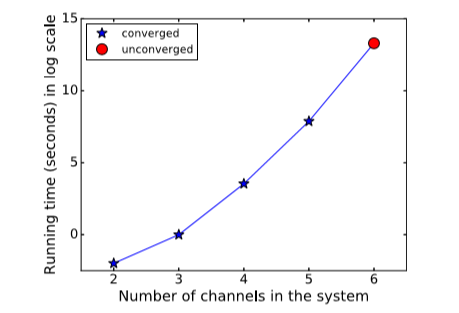
\includegraphics[width = 1.0\textwidth]{附录图1}
	\caption{fig1}
\end{figure}

 run-time as we increase the number of channels in the system. When the number of channels is higher than 5, we find that the POMDP solver can not converge after a long interval, and it gets terminated when the run-time exceeds the time limit. All these factors make it impossible to find the optimal solution to the problem in general, and many existing works [8]–[10], [17]–[21] attempt to address this challenge ofprohibitive computation by considering either simpler models or approximation algorithms.

\section*{  MYOPIC POLICY AND WHITTLE INDEX   }
In the domain of dynamic multichannel access, there are many existing works on finding the optimal/near-optimal policy with low computation cost when the channels are independent and system statistics (P) is known. The Myopic policy and the Whittle Index policy are two effective and easy-to-implement approaches for this setting.

A Myopic policy only focuses on the immediate reward obtained from an action and ignores its effects in the future. Thus the user always tries to select a channel which gives the maximized expected immediate reward. The Myopic policy is not optimal in general. Researchers in [8] and [ 9] have studied its optimality when N channels are independent and statistically identical Gilbert-Elliot channels that follow the same 2-state Markov chain with the transition matrix.In addition, the Myopic policy has a simple robust structure that follows a round-robin channel selection procedure.

When channels are independent, the dynamic multichannel access problem can also be considered as a restless multiarmed bandit problem (RMAB) if each channel is treated as an arm. An index policy assigns a value to each arm based on its current state and chooses the arm with the highest index at each time slot. The index policy is not guaranteed to be optimal in general. 

In [10], the Whittle Index is obtained in closed-form for the case when P is known and all channels are independent but may follow different 2-state Markov chain models. In thespecial case when all channels are identical, it is shown to coincide with the above-described Myopic policy.
\begin{figure}[h]
	\centering
	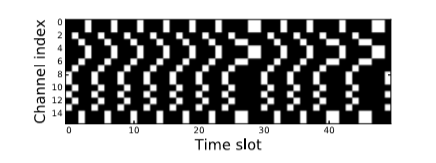
\includegraphics[width = 1.0\textwidth]{附录图2}
	\caption{fig2}
\end{figure}
When channels are correlated, the Whittle Index cannot be defined and thus the Whittle Index policy cannot be directly applied to our problem.Nevertheless, as a baseline in our evaluations, to leverage its simplicity, we propose an heuristic that ignores the correlations among channels and uses the joint transition matrix P and Bayes’ Rule to compute the 2-state Markov chain for each individual channel. Once each channel model is found, we can apply the Whittle Index policy accordingly. 

The Myopic policy and the Whittle Index policy are easy to implement in practice and have polynomial run-time, however they achieve optimality only under certain conditions when channels are independent. Moreover, both policies require prior knowledge of the system dynamics, which is hard to obtain beforehand. However, to the best of our knowledge, there is no easy-to-implement policy applicable to the general case where channels are correlated and the system dynamics are unknown — thus a new approach is needed.

\section*{  DEEP REINFORCEMENT LEARNING FRAMEWORK    }
When channels are correlated and system dynamics are unknown,there are two main approachesto tackle the dynamic multichannel access problem:  The model-based approach is less favored since the user’s limited observation capability may result in a bad system model estimation. Even worse, even if the system dynamics is well estimated, solving a POMDP in a large state space is always a bottleneck as the dynamic programming method has exponential time complexity and the heuristic approaches do not have any performance guarantee. All these challenges motivate us to follow the model-free approach, which, by incorporating the idea of Reinforcement Learning, can learn directly from observations without the necessity of finding an estimated system model and can be easily extended to very large and complicated systems.In the context of the dynamic multichannel access, the problem can be converted to an MDP when considering the belief space, and Q-learning can be applied consequently. However,this approachis impractical since the belief update is maintainedby knowingthesystem transitionmatrixP a-priori, which is hardly available in practice. Instead, we apply Qlearning by directly considering the history of observations and actions. We define the state for the Q-learning at time slot t as a combination of historical selected channels as well as their observed channel conditions over previous M time slots, And intuitively, the more historical information we consider the better Q-learning can learn.

Q-learning works well when the problem’s state space is small, as a look-up table can be used to update Q values. But this is impossible when the state space becomes large. The state space size in this work grows exponentially as we use a combination of M vectors of length N to represent historical observations and actions for a system with N 2-state channels over past M time slots. M is required to be large so that Q-learning can capture enough information for learning.Even worse, since many states are rarely visited, their corresponding Q-values are seldom updated. This causes Q learning to take a very long time to converge.Motivated by its success in other domains [5], we adopt the deep Q-Network approach to address the very large state space. DQN takes the state-action pair as input and outputs the corresponding Q-value. Q-network updates its weights θ at each iteration i to minimize the loss function $Q^{*}\left ( s,a \right )=\sum _{{s}'}P\left ( {s}'\mid s,a \right )\left ( R\left ( s,a,{s}' \right ) +\gamma\max _{{a}'}Q^{*}\left ( {s}' ,{a}'\right )\right )$.

To study the performance of DQN, we first consider a correlated channel model that we refer to as fixed-pattern channel switching, in which all the N channels in the system can be divided into several independentsubsets and these subsets take turns to be activated following a fixed pattern. Specifically, we assume all channels in one currently activated subset are good and all channels in inactivated subsets are bad. At each time slot, with a known probability the next following subset is activated, and with probability 1−p the current subset remains activated. We assume the activation order of the subsets is known, fixed, and will not change over time. In this special case, the optimal policy can be found analytically and is summarized in Theorem 1, providing a baseline to evaluate the performance of DQN implementation in the next section. 

\section*{  EXPERIMENT AND EVALUATION OF LEARNING FOR UNKNOWN FIXED-PATTERN CHANNEL SWITCHING     }
We present details of our DQN implementation and then evaluate its performance on the fixed-pattern switching pattern model, comparing it to the optimal policy, through experiments.

We design a DQN by following the Deep Q-learning with Experience Replay Algorithm [5] and implement it in TensorFlow [24]. The structure of our DQN is finalized as a fully connected neural network with each of the two hidden layers containing 200 neurons.1 The activation function of each neuron is Rectified Linear Unit (ReLU),The inputofthe DQN is defined as the combination of previous actions and observations over previous M time slots

In our experiments, we considered different situations: single good channel or multiple good channels, sequential switching or arbitrary switching, and observe that DQN can achieve the optimal performance in all situations. Due to the space constraint, we only present results on the multiple good channels situation, and refer the reader to [23] for more results on other situations. In this section, we investigate the fixed-pattern channel switching model with 16 channels are evenly divided into several subsets that take turns to become available with a switching probability fixed at p = 0.9. In Fig. 2, we provide a pixel illustration to visualize how the states of channels change in a multiple good channels situation over 50 time slots, where a white cell indicates the corresponding channel is good at the corresponding time. We compare the DQN with two other policies: the Whittle Index heuristic policy and the optimal policy with known system dynamics from Section VI. The optimal policy has full knowledge of the system dynamics and serves as a performance upper bound. In the Whittle Index heuristic, the user assumes all channels are independent and observes each channel individually for 10,000 time slots to estimate its 2-state Markov chain transition matrix.
\begin{figure}[h]
	\centering
	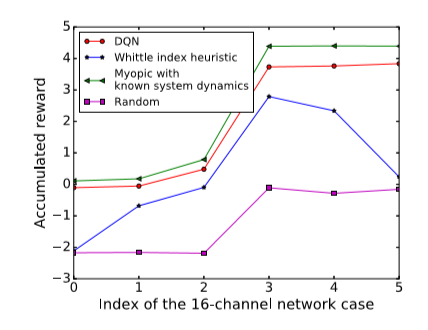
\includegraphics[width = 1.0\textwidth]{附录图3}
	\caption{fig3}
\end{figure}

We vary the number of channels in a subset as 1, 2, 4 and 8 in the experiment, and present the experimental results in Fig. 3. The 16 channels in the system are in order and the subsets are activated in a sequential round-robin order in the upper graph in Fig. 3, while the channels are arranged arbitrarily and the activation order of subsets is also arbitrary in the bottom graph in Fig. 3. As can be seen, DQN remains robust and achieves the same optimal performance in all cases as the optimal policy and performs significantly better than the Whittle Index heuristic. This shows that DQN can implicitly learn the system dynamics includingthe correlation among channels, and finds the optimal policy accordingly. On the contrary, the Whittle Index heuristic simply assumes the channels are independent and is not able to find or make use of the correlation among channels. Moreover, the training time decreases as the number of good channels increases. This is because there is more chance to find a good channel when more good channels are available at a time slot, and the learning process becomes easier so that the DQN agent can take less time exploring and is able to find the optimal policy more quickly. This also explains why Whittle Index heuristic performs better when there are more good channels available.

We consider a highly correlated scenario. In a 16-channel system, we assume only two or three channels are independent, and other channels are exactly identical or opposite to one of these independent channels. In addition to the Whittle Index heuristic, we also compare DQN with a Random Policy in which the user randomly selects one channel with equalprobability at each time slot. Since the optimal policy is computationally prohibitive, we implement the Myopic policy instead as a genie(knowingthe system statistics a-priori) since it is simple, robust and can achieve an optimal performance in certain situations. In Fig. 4 we present the performance of all four policies: (i) DQN, (ii) Random, (iii) Whittle Index heuristic, and (iv) Myopic policy with known P. In the first three cases (x-axis 0, 1 and 2), the correlation coefficient ρ is fixed as 1 and in the last three cases (x-axis 3, 4 and 5), ρ is fixed as−1. We also vary the set of correlated channels to make cases different. The Myopic policy in the first three cases is optimal, and in the last three cases is conjectured to be near-optimal. As shown in Fig. 4, the Myopic policy, which is implemented based on the full knowledge of the system, is the best among all six cases and serves as an upper bound. DQN provides a performance very close to the Myopic policy without any knowledge of the system dynamics. The Whittle Index policy performs worse than DQN in all cases.
\begin{figure}[h]
	\centering
	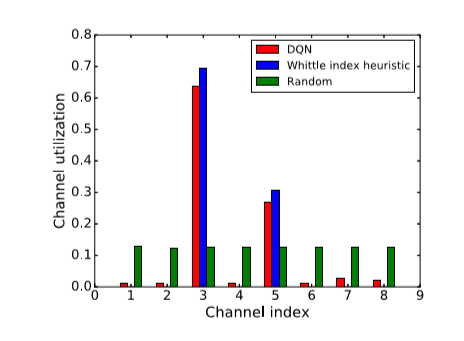
\includegraphics[width = 1.0\textwidth]{附录图4}
	\caption{fig4}
\end{figure}
\section*{  CONCLUSION AND FUTURE WORK   }

In this paper, we have considered the dynamic multichannel access problem in a more general and practical scenario when channels are correlated and system statistics is unknown. The problem is an unknown POMDP without any tractable solution, and we have applied an end-to-end DQN approach that directly utilizes historical observations and actions to find the access policy via online learning. In the fixed-pattern channel switching, we have analytically found the optimal access policy with known system statistics and full observation ability. Through simulations, we have shown DQN is able to achieve the same optimal performance even without any prior knowledge. We have also shown from both simulations and real data trace that DQN can achieve near-optimal performance in more complex scenarios. In addition, we have designed an adaptive DQN and shown through numerical simulations that it can detect system changes and re-learn in non-stationary dynamic environments.

There are a number of open directions suggested by the present work. First, we plan to apply the DQN framework to consider more realistic and complicated scenarios such as multi-user, multi-hop and simultaneous transmissions in WSNs. The framework of DQN can be directly extended to consider these practical factors in a simple way. For example, in the situation of multiple users, to avoid interference and collisions among users, we can adopt a centralized approach: assuming there is a centralized controller that can select a subset of non-interferingchannels at any time slot, and assign one to each user to avoid a collision. By redefining the action as selecting a subset of non-interferingchannels, the DQN framework can be directly used for this multi-user scenario. As the action space becomes large when selecting multiple channels, the current DQN structure requires careful re-design and may require very long training interval before finding a reasonable solution. Instead, we use the same DQN structure as that in Section VII and consider the multiple-users situation in a smaller system that contains 8 channels where at any time slot 6 channels become good and channel conditions change in a round-robin pattern. The number of users varies from 2 to 4. As is shown in Fig. 8, DQN can still achieve a good performance in the multiple-user case. Other deep reinforcement learning approaches, such as Deep Deterministic PolicyGradient (DDPG) [27], will be studied in future to tackle the large action space challenge. Second, when the number of users in the network becomes large, the above proposed centralized approach becomes too computationally expensive. In future, we plan to study a more practical distributed approach where each user can learn a channel selection policy independently. One intuitive idea is to implement a DQN at each user independently. Then users can learn their channel selection policies parallelly, and avoid interference and conflicts by making proper channel-selection decisions based on the information gained from observations and rewards. However, whether a good or optimal policy can be learned, and whether an equilibrium exists are unknown and need further investigation.we encourage the networking community to work together to create an open source dataset that contains different practical channel access scenarios so that researchers can benchmark the performance of different approaches. We have published all the channel access environments and real data trace considered in this work.
This might serve as an useful benchmark dataset for researchers to use.


\section*{References}

\begin{figure}[h]
	\centering
	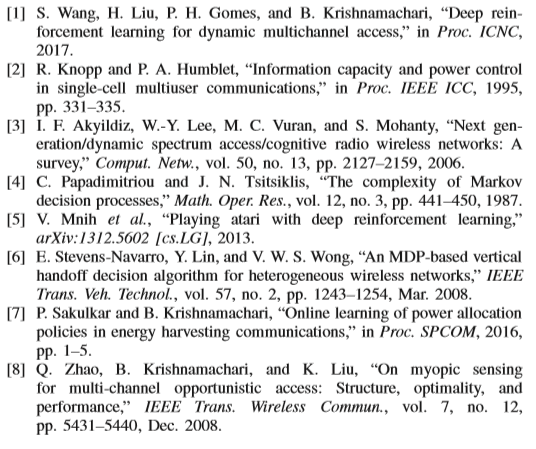
\includegraphics[width = 1.0\textwidth]{附录参考文献1}
	\caption{附录参考文献1}
\end{figure}

\begin{figure}[h]
	\centering
	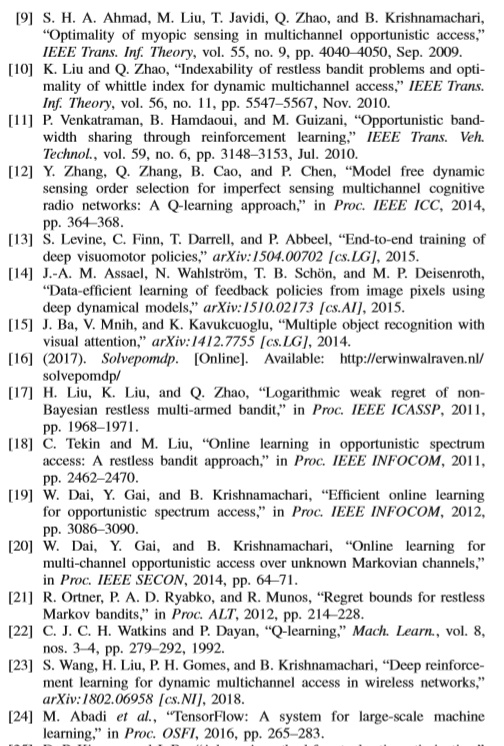
\includegraphics[width = 1.0\textwidth]{附录参考文献2}
	\caption{附录参考文献2}
\end{figure}
%\begin{translationbib}
%\item Donald E. Knuth. The \TeX book. Addison-Wesley, 1984. ISBN: 0-201-13448-9
%\item Paul W. Abrahams, Karl Berry and Kathryn A. Hargreaves. \TeX\ for the
%  Impatient. Addison-Wesley, 1990. ISBN: 0-201-51375-7
%\item David Salomon. The advanced \TeX book.  New York : Springer, 1995. ISBN:0-387-94556-3
%\end{translationbib}

\chapter{外文资料的调研阅读报告或书面翻译}

\title{无线网络中动态多通道访问的深度强化学习}

{\heiti 摘要:} 我们考虑一个动态的多通道访问问题,其中多个相关的通道遵循未知的联合马尔可夫模型,并且用户选择通道来传输数据。目的是找到一种政策,以使成功传输的预期长期数量最大化。该问题被表述为具有未知系统动力学的部分可观察到的马尔可夫决策过程。为了克服未知动力学和过高计算的挑战,我们应用了强化学习的概念并实现了深度Q网络(DQN)。我们首先研究具有已知系统动态特性的固定模式信道切换的最佳策略,并通过仿真显示DQN可以在不了解系统统计信息的情况下达到相同的最佳性能。然后,我们通过更一般的模拟以及实际数据跟踪,将DQN的性能与近视策略和基于Whittle索引的启发式方法进行比较,并显示DQN在更复杂的情况下可达到最佳性能。最后,我们提出了一种自适应DQN方法,该方法具有在时变情况下适应其学习的能力。

\section*{ 介绍 }
先前的工作[2],[3]表明,动态频谱访问是提高无线网络频谱利用率和满足更大容量需求的关键之一。 在认知无线电研究的背景下,标准假设是次要用户可以搜索和使用其主要用户(PU)并未使用的空闲信道。 虽然先前的工作通常假设一个简单的独立信道(或PU活动)模型,但实际上,外部干扰会导致无线网络中的信道高度相关,因此需要设计动态多信道访问中的新算法和方案来解决 这个挑战。
我们在这项工作中考虑了具有N个相关通道的多通道访问问题。 每个通道具有两个可能的状态:好或坏,并且它们的联合分布遵循$2^{N}$状态马尔可夫模型。 有一个用户(无线节点)在每个时隙选择一个通道来传输数据包。 如果选择的频道处于良好状态,则传输成功; 否则,传输失败。 目标是随着时间的推移获得尽可能多的成功传输。 由于用户只能在每个时隙中感测到他选择的频道,因此无法完全观察到可用的系统。 通常,可以将问题表述为部分可观察到的马尔可夫决策过程(POMDP),这是PSPACE难解的,要找到确切的解决方案,最著名的解决方案需要指数计算复杂性[4]。 更糟糕的是,联合马尔可夫模型的参数可能不是先验的。

我们研究了机器学习领域中深度强化学习(尤其是深度Q学习)的使用,以此作为一种在未知环境中进行学习并克服令人望而却步的计算要求的方法。 通过将深度学习与Q学习集成在一起,深度Q学习或深度Q网络(DQN)[5]可以使用状态作为输入,估计Q值作为输出的深度神经网络,以有效地学习高维,大状态空间的策略 问题。我们实现了一种DQN,该DQN可以通过在线学习来找到频道访问策略。 这种DQN方法能够处理大型系统,并且可以直接从历史观察中找到更好甚至最佳的策略,而无需知道先验的系统动力学。

本文的其余部分安排如下。 第二节介绍了相关工作。 第三节阐述了当信道潜在相关时的动态多信道访问问题。 第四部分介绍了基于近视和Whittle索引的启发式方法来解决此问题。 第五部分介绍了DQN框架。 第六节介绍了有关已知固定模式信道切换的最佳策略研究,第七节通过仿真显示DQN可以实现最佳性能。 第八节显示了考虑综合数据集和基于试验床的数据集的评估结果。 第九节介绍了一种自适应DQN方法,最后,第十节总结了我们的工作。

\section*{  相关工作与问题建模  }
动态多信道访问问题已被广泛研究。但是与许多决策问题不同,例如垂直切换[6]和功率分配[7],它可以
如果将其建模为MDP,则将动态多通道问题建模为POMDP,因为通道通常是(两个状态的)马尔可夫链,并且用户只有部分观察力。寻找最佳的信道访问策略需要指数级的时间和空间复杂度。当频道是独立的且分布均匀(即i.d.)时,近视策略在某些条件下显示为最佳[8],[9]。但是,当渠道相关或遵循不同的分布时,近视策略不具有任何性能保证。当通道独立但可以遵循不同的马尔可夫链时,可以将动态多通道访问问题建模为不安多臂匪徒问题(RMAB)。 Whittle索引策略在[10]中引入,与近视策略具有相同的简单半通用结构和最优结果。数值结果还表明,当渠道不相同时,Whittle指数策略可以实现接近最佳的性能,但是当渠道相关时,Whittle指数方法不适用,这是我们的工作重点。

近年来,一些工作开始集中于更实际和更复杂的问题,即系统统计信息未知且通道相关。 Q学习是一种无模型的方法,可以直接通过在线学习来学习策略,因此被广泛使用。 Venkatraman等。 [11]将Q学习应用于设计信道感测序列,而在[12]中则表明Q学习还可以解决不完善的感测问题。 所有这些工作都假定系统状态是完全可观察的,并将问题表述为MDP,从而显着减少了状态空间。 相反,由于部分观察的局限性,我们的问题落入了POMDP的框架中,并且其较大的状态空间使其无法维护简单的查询Q表来更新Q值。 需要能够找到Q值近似值的新方法来解决大空间挑战。

强化学习(包括Q学习)已与先进的机器学习技术集成在一起,以解决困难的高维问题[13] – [15]。 2013年,Google DeepMind使用了称为DQN的深度神经网络来逼近Q学习中的Q值,从而克服了传统查找表方法的局限性,并提供了一种端到端的方法以允许代理人学习 政策的观察。 据我们所知,我们是动态多通道访问领域中DQN的第一个研究和实现。

考虑一个动态多通道访问问题,其中有一个用户动态地从N个通道中选择一个。 在每个时隙的开始,用户选择一个通道来感测和发送数据包。 如果信道质量良好,则传输成功并且用户获得正奖励(+1),否则用户传输失败并且存在负奖励(-1)。 目的是设计一种能够最大化预期长期回报的政策。 

为了建模跨渠道的关联,整个系统被描述为 $2^{N}$ 马尔可夫链. 这里,让马尔可夫链的状态空间为$S=\left\{S_{1},\cdots,S_{2^{N}}\right\}$,每个状态 $S_{i}$  是一个长度为N的向量,其中是信道k状态的二进制表示形式:好(1)或坏(0)。
马尔可夫链的跃迁表示为P。由于用户只能在每个时隙的开头感知一个频道,因此无法观察到所有频道的完整状态。 但是,用户可以根据其感测决策和观察结果推断系统状态的分布。 因此,动态多信道接入问题属于POMDP的通用框架。$\Omega \left ( t \right )=\left [ \omega _{S_{1}} \left ( t \right ),\cdots,\omega _{S_{2^{N}}} \left ( t \right )\right ]$ , 代表用户维护的置信向量,在给出所有先前决策和观察结果的情况下系统处于状态的条件概率。
然后,基于此观察结果,用户可以在时隙t处更新置信向量,如下所示:
\begin{equation}\tag*{1}
\hat{\omega }_{S_{i}}\left ( t \right )=\left\{
\begin{aligned}
\frac{\omega _{s_{i}\left ( t \right )}\mathbb{I}\left ( S_{ik}\left ( t \right ) =1\right )}{\sum_{i=1}^{2^{N}}\omega _{s_{i}\left ( t \right )}\mathbb{I}\left ( S_{ik}\left ( t \right ) =1\right )}& & a(t)=k,o(t)=1\\
\frac{\omega _{s_{i}\left ( t \right )}\mathbb{I}\left ( S_{ik}\left ( t \right ) =1\right )}{\sum_{i=0}^{2^{N}}\omega _{s_{i}\left ( t \right )}\mathbb{I}\left ( S_{ik}\left ( t \right ) =0\right )}& & a(t)=k,o(t)=0
\end{aligned}
\right.
\end{equation}
我们的目标是找到一种感应政策 $\pi^{*}$ 得到在无限时间内最大化预期的累积折扣奖励
\begin{equation}\tag*{2}
\pi ^{*}= \underset{\pi }{\arg \max}\mathbb{E}_{\pi}\left [ \sum_{t=1}^{\infty }\gamma ^{t-1} R_{\pi\left ( \Omega \left ( t \right ) \right )}\left ( t \right )\mid \Omega \left ( 1 \right )\right ]
\end{equation}

由于动态多通道访问问题是POMDP,因此可以通过考虑其置信空间并求解增强的MDP(例如,通过值迭代)来找到最佳的感知策略$\pi^{*}$,但是置信向量的维数在指数上较大。 通道数。 更糟糕的是,连续信念空间的无限大小以及当前操作对未来奖励的影响使POMDP PSPACE难以解决,与NP难解决的问题相比,在多项式时间内难以解决[4]。 为了举例说明解决此类POMDP问题的时间复杂性,我们以已知的系统动力学模拟了多通道访问问题,并使用称为POMDP求解器[16]来找到其最佳解决方案。 在图1中,我们显示了
\begin{figure}[h]
	\centering
	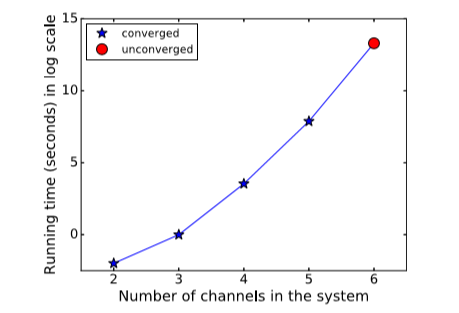
\includegraphics[width = 1.0\textwidth]{附录图1}
	\caption{fig1}
\end{figure}

运行时间,因为我们增加了系统中的通道数。 当通道数大于5时,我们发现POMDP求解器在长时间间隔后无法收敛,并且在运行时间超过时间限制时终止。 所有这些因素使得不可能找到一般问题的最佳解决方案,并且许多现有的工作[8]到[10],[17]到[21]试图通过考虑更简单的模型或近似来解决这一禁止计算的挑战算法。

\section*{ 传统算法  }
在动态多通道访问领域,当通道独立且系统统计数(P)已知时,已有许多工作以较低的计算成本来寻找最优/近最优策略。 近视策略和Whittle索引策略是此设置的两种有效且易于实现的方法。

近视策略仅关注从动作中获得的即时奖励,而忽略了其将来的影响。 因此,用户总是尝试选择给出最大化的预期立即奖励的频道。 通常,近视策略不是最佳的。 [8]和[9]中的研究人员研究了N个通道是独立的且统计上相同的吉尔伯特-艾略特通道,它们遵循具有过渡矩阵的相同2状态马尔可夫链时的最优性。此外,近视策略具有简单的鲁棒结构 遵循循环信道选择过程。

当通道是独立的时,如果将每个通道视为一个分支,则动态多通道访问问题也可以视为不安多臂强盗问题(RMAB)。 索引策略根据每个分支的当前状态为其分配一个值,并在每个时隙中选择索引最高的分支。 通常,不能保证索引策略是最佳的。

在[10]中,对于已知P且所有通道都是独立的但可能遵循不同的2状态马尔可夫链模型的情况,以封闭形式获得Whittle指数。 在所有通道都相同的特殊情况下,这表明与上述近视策略一致。
\begin{figure}[h]
	\centering
	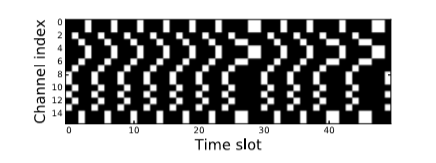
\includegraphics[width = 1.0\textwidth]{附录图2}
	\caption{fig2}
\end{figure}
当信道相关时,无法定义Whittle指数,因此无法将Whittle指数政策直接应用于我们的问题。但是,作为评估的基准,为了利用其简单性,我们提出了一种启发式方法,该方法忽略了渠道之间的相关性。 使用联合过渡矩阵P和贝叶斯规则为每个单独的通道计算2状态马尔可夫链。 找到每个渠道模型后,我们可以相应地应用Whittle Index策略。

近视策略和Whittle索引策略在实践中易于实现并且具有多项式运行时,但是它们仅在通道独立的特定条件下才能实现最优。 而且,这两种策略都需要先验的系统动力学知识,而这是很难事先获得的。 但是,据我们所知,没有适用于通行相关且系统动态未知的一般情况的易于实现的策略,因此需要一种新的方法。

\section*{  深度强化学习框架    }
当通道相关且系统动态未知时,有两种主要的方法可以解决动态多通道访问问题:基于模型的方法不太受青睐,因为用户有限的观察能力可能会导致不良的系统模型估计。甚至更糟的是,即使系统动力学得到了很好的估计,在大状态空间中解决POMDP始终是瓶颈,因为动态编程方法具有指数级的时间复杂度,并且启发式方法没有任何性能保证。所有这些挑战促使我们采取无模型方法,该方法通过整合强化学习的思想,可以直接从观察中学习,而无需寻找估计的系统模型,并且可以轻松地扩展到非常大而复杂的系统。在动态多通道访问的上下文中,考虑到置信空间后,可以将问题转换为MDP,从而可以应用Q学习。但是,这种方法是不切实际的,因为通过了解系统转换矩阵P来维持信念更新,而这在实践中几乎是不可用的。相反,我们通过直接考虑观察和行动的历史来应用Qlearning。我们将时隙t处的Q学习状态定义为历史选定通道及其在先前M个时隙中观察到的通道状况的组合。从直觉上讲,我们认为越多的历史信息可以更好地学习Q学习。

当问题的状态空间较小时,Q学习效果很好,因为可以使用查询表来更新Q值。 但是,当状态空间变大时,这是不可能的。 由于我们使用长度为N的M个向量的组合来表示过去M个时隙中具有N个2状态通道的系统的历史观测值和动作,因此这项工作中的状态空间大小呈指数增长。 M必须很大,以便Q学习可以捕获足够的学习信息。更糟糕的是,由于很少访问许多状态,因此很少更新其对应的Q值。 这导致Q学习需要很长时间才能收敛。受其在其他领域的成功的推动[5],我们采用深度Q网络方法来处理非常大的状态空间。 DQN将状态操作对作为输入并输出相应的Q值。 Q网络在每次迭代i时都会更新其权重$\sigma$以最小化损失函数$Q^{*}\left ( s,a \right )=\sum _{{s}'}P\left ( {s}'\mid s,a \right )\left ( R\left ( s,a,{s}' \right ) +\gamma\max _{{a}'}Q^{*}\left ( {s}' ,{a}'\right )\right )$.

为了研究DQN的性能,我们首先考虑一个相关的信道模型,我们将其称为固定模式信道切换,其中系统中的所有N个信道都可以分为几个独立的子集,并且这些子集轮流被激活。 固定模式。 具体来说,我们假设一个当前激活的子集中的所有通道都是好通道,而未激活的子集中的所有通道都不好。 在每个时隙,以已知的概率激活下一个后续子集,以概率1-p激活当前子集。 我们假设子集的激活顺序是已知的,固定的,并且不会随时间变化。 在这种特殊情况下,可以通过分析找到最佳策略,并在定理1中对其进行了总结,在下一节中提供了基准来评估DQN实施的性能。

\section*{ 未知固定模式通道切换的学习实验和评估  }
我们介绍DQN实现的详细信息,然后通过固定模式切换模式模型评估其性能,并将其与最佳策略进行比较。

我们通过使用体验重放算法[5]进行深度Q学习来设计DQN,并在TensorFlow [24]中实现它。 我们的DQN的结构最终确定为一个完全连接的神经网络,两个隐藏层中的每一层都包含200个神经元。1每个神经元的激活函数为ReLU,DQN的输入定义为先前动作的组合 和对前M个时隙的观察。

在我们的实验中,我们考虑了不同的情况:单个良好通道或多个良好通道,顺序切换或任意切换,并观察到DQN可以在所有情况下均达到最佳性能。由于篇幅所限,我们仅在多个良好渠道的情况下给出结果,而将读者推荐给[23]以获取其他情况下的更多结果。在本节中,我们研究固定模式的信道切换模型,其中将16个信道均匀地分成几个子集,这些子集轮流可用,切换概率固定为p = 0.9。在图2中,我们提供了一个像素图,以可视化方式显示在50个时隙内多个良好通道情况下通道状态如何变化,其中白色单元格指示相应通道在相应时间处于良好状态。我们将DQN与其他两个策略进行比较:Whittle指数启发式策略和具有第六部分已知系统动态的最优策略。最佳策略完全了解系统动力学,并充当性能上限。在Whittle Index启发式方法中,用户假定所有通道都是独立的,并在10,000个时隙中分别观察每个通道,以估计其2状态马尔可夫链跃迁矩阵。
\begin{figure}[h]
	\centering
	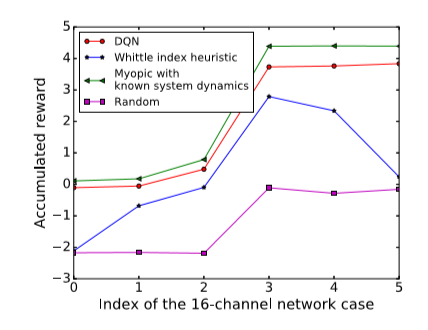
\includegraphics[width = 1.0\textwidth]{附录图3}
	\caption{fig3}
\end{figure}

在实验中,我们将一个子集中的通道数更改为1、2、4和8,并在图3中显示了实验结果。系统中的16个通道是按顺序排列的,并且这些子集在连续的回合中被激活。在图3的上图中,罗宾顺序是任意的,而通道在图3的下图中是任意排列的,子集的激活顺序也是任意的。可以看出,DQN保持鲁棒性,并在图3中达到相同的最佳性能。所有情况都是最佳策略,并且其性能比Whittle Index启发式方法好得多。这表明DQN可以隐式学习系统动力学,包括通道之间的相关性,并据此找到最佳策略。相反,Whittle指数试探法简单地假设通道是独立的,并且无法找到或利用通道之间的相关性。而且,训练时间随着良好频道数量的增加而减少。这是因为,如果在某个时隙有更多的良好频道可用,则有更多的机会找到一个良好的频道,并且学习过程变得更加容易,因此DQN代理可以花费更少的时间进行探索,并且能够更快地找到最佳策略。这也解释了为什么在有更多可用渠道时,Whittle Index启发式方法的效果更好。

我们考虑一个高度相关的场景。在16通道系统中,我们假设只有两个或三个通道是独立的,其他通道与这些独立通道之一完全相同或相对。除了Whittle Index启发式算法外,我们还将DQN与随机策略进行比较,在随机策略中,用户在每个时隙随机选择一个概率均等的通道。由于最佳策略在计算上是禁止的,因此我们将近视策略作为精灵来实现(知道系统统计信息是先验的),因为它简单,健壮并且可以在某些情况下实现最佳性能。在图4中,我们展示了所有四种策略的性能:(i)DQN,(ii)随机,(iii)Whittle指数启发式和(iv)具有已知P的近视策略。在前三种情况下(x轴0 ,1和2),相关系数ρ固定为1,在后三种情况(x轴3、4和5)中,ρ固定为-1。我们还更改了相关通道的集合,以使情况有所不同。在前三个案例中,近视策略是最佳的,而在后三个案例中,近视策略被认为是最佳的。如图4所示,基于系统的全部知识而实现的近视策略在所有六个情况中都是最好的,并作为上限。 DQN提供的性能非常接近于近视策略,而无需任何系统动力学知识。在所有情况下,Whittle指数政策的表现都比DQN差。
\begin{figure}[h]
	\centering
	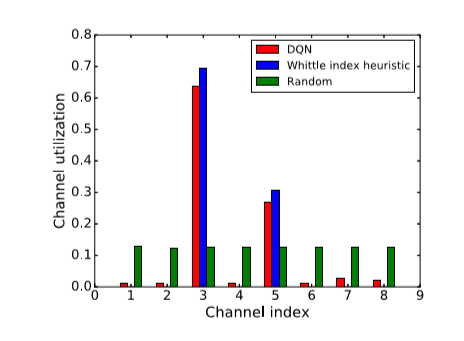
\includegraphics[width = 1.0\textwidth]{附录图4}
	\caption{fig4}
\end{figure}
\section*{  结论和展望   }

在本文中,我们考虑了在通道相关且系统统计信息未知的情况下,在更通用和更实际的情况下动态多通道访问问题。 问题是一个未知的POMDP,没有任何可解决的解决方案,我们已经采用了一种端到端DQN方法,该方法直接利用历史观察和操作来通过在线学习找到访问策略。 在固定模式信道切换中,我们已经分析地找到了具有已知系统统计信息和完整观察能力的最佳访问策略。 通过仿真,我们证明了DQN即使没有任何先验知识也能够实现相同的最佳性能。 我们还从仿真和实际数据跟踪中都表明,DQN在更复杂的情况下可以实现近乎最佳的性能。 此外,我们设计了自适应DQN,并通过数值模拟表明它可以检测系统变化并在非平稳动态环境中重新学习。

当前的工作建议了许多开放的方向。首先,我们计划应用DQN框架来考虑更现实,更复杂的场景,例如WSN中的多用户,多跳和同时传输。 DQN的框架可以直接扩展,以简单的方式考虑这些实际因素。例如,在有多个用户的情况下,为避免用户之间的干扰和冲突,我们可以采用集中式方法:假设有一个集中式控制器,该控制器可以在任何时隙中选择一个无干扰信道的子集,并为每个时隙分配一个用户避免碰撞。通过将动作重新定义为选择无干扰信道的子集,DQN框架可直接用于此多用户方案。当选择多个通道时,由于动作空间变大,当前的DQN结构需要仔细的重新设计,并且在找到合理的解决方案之前可能需要很长的训练间隔。取而代之的是,我们使用与第七节相同的DQN结构,并考虑在包含8个通道的较小系统中的多用户情况,该系统在任何时隙中6个通道变好,并且通道条件以循环模式改变。用户数从2到4不等。如图8所示,在多用户情况下DQN仍然可以实现良好的性能。未来还将研究其他深度强化学习方法,例如深度确定性策略梯度(DDPG)[27],以应对大型行动空间挑战。其次,当网络中的用户数量变大时,以上提出的集中式方法在计算上变得太昂贵。将来,我们计划研究一种更实用的分布式方法,其中每个用户可以独立学习频道选择策略。一个直观的想法是在每个用户处独立实现DQN。然后,用户可以并行学习其频道选择策略,并根据从观察和奖励中获得的信息做出适当的频道选择决策,从而避免干扰和冲突。但是,是否可以学习一个好政策还是最优政策以及是否存在均衡尚不明确,需要进一步研究。我们鼓励网络社区共同创建一个包含不同实际渠道访问场景的开源数据集,以便研究人员可以进行基准测试不同方法的效果。我们已经发布了这项工作中考虑的所有通道访问环境和实际数据跟踪。
这可能是供研究人员使用的有用基准数据集。

